 %=======================================================================
%  LABORATORIO N.o 1 - MI PRIMER CIRCUITO
%  Curso : Circuitos Electronicos  (2026-2)
%  UCSP  - Facultad de Ingenieria - Ing. Electronica y de Telecomunicaciones
%  Docente: Ebert San Roman Castillo
%
%  Version 2 - Revision tecnica y de estilo.
%  Los bloques marcados como "Nota tecnica", "Seguridad", "Ejemplo de
%  diseno" y "Verificacion experimental" son ANADIDOS a la guia original;
%  el resto del texto conserva el contenido del documento .doc de origen.
%
%  Compilar:  xelatex Laboratorio_1.tex    (dos veces)
%=======================================================================
\documentclass[11pt,a4paper]{article}

%------------------------------------------------------------- idioma
% Compilar con XeLaTeX (no con pdflatex): Trebuchet MS es una fuente TrueType
% del sistema y solo fontspec, bajo XeLaTeX o LuaLaTeX, sabe cargarla.
% inputenc y fontenc se omiten a proposito: XeLaTeX trabaja en UTF-8 de forma
% nativa y esos paquetes dan error con este motor.
\usepackage{fontspec}
\setmainfont{Trebuchet MS}[
  Path            = C:/Windows/Fonts/,
  Extension       = .ttf,
  UprightFont     = trebuc,
  BoldFont        = trebucbd,
  ItalicFont      = trebucit,
  BoldItalicFont  = trebucbi,
  Ligatures       = TeX
]
\usepackage[spanish,es-nodecimaldot]{babel}
\usepackage{microtype}

%----------------------------------------------------------- geometria
\usepackage[left=2.4cm,right=2.4cm,top=3.1cm,bottom=2.6cm,headheight=30pt,
            footskip=1.2cm]{geometry}

%------------------------------------------------------------ graficos
\usepackage{graphicx}
\usepackage{float}
\usepackage{placeins}
\usepackage[font=small,labelfont=bf,labelsep=period]{caption}
\graphicspath{{imagenes/}}

%-------------------------------------------------------------- tablas
\usepackage{array}
\usepackage{tabularx}
\usepackage{booktabs}
\usepackage{multirow}

%----------------------------------------------------- matematicas / SI
\usepackage{amsmath,amssymb}
\usepackage{siunitx}
\sisetup{
  output-decimal-marker = {,},
  per-mode              = symbol,
  range-phrase          = { a },
  range-units           = single,
  detect-weight         = true,
  detect-family         = true
}
\DeclareSIUnit{\sample}{S}          % muestra (para MS/s)

%--------------------------------------------------------------- listas
\usepackage{enumitem}
\setlist[itemize]{itemsep=3pt,topsep=4pt,parsep=0pt}
\setlist[enumerate]{itemsep=8pt,topsep=4pt,parsep=0pt}

%--------------------------------------------------------------- cajas
\usepackage[most]{tcolorbox}
\usepackage{pgffor}

\newtcolorbox{notatec}[1]{enhanced,breakable,
  colback=blue!3!white, colframe=blue!55!black,
  fonttitle=\bfseries\small, title={Nota técnica --- #1},
  boxrule=0.6pt, arc=2pt, left=6pt,right=6pt,top=4pt,bottom=4pt}

\newtcolorbox{seguridad}[1]{enhanced,breakable,
  colback=red!3!white, colframe=red!60!black,
  fonttitle=\bfseries\small, title={Seguridad --- #1},
  boxrule=0.6pt, arc=2pt, left=6pt,right=6pt,top=4pt,bottom=4pt}

\newtcolorbox{ejemplo}[1]{enhanced,breakable,
  colback=green!3!white, colframe=green!45!black,
  fonttitle=\bfseries\small, title={Ejemplo de diseño --- #1},
  boxrule=0.6pt, arc=2pt, left=6pt,right=6pt,top=4pt,bottom=4pt}

%------------------------------------------------------------ comandos
% Lineas punteadas para respuestas del alumno: \lineasresp{n}
\newcommand{\lineasresp}[1]{%
  \par\vspace{6pt}%
  \foreach \i in {1,...,#1}{\noindent\rule{\linewidth}{0.4pt}\par\vspace{11pt}}%
}

%---------------------------------------------------- encabezado / pie
\usepackage{fancyhdr}
\pagestyle{fancy}
\fancyhf{}
\fancyhead[L]{\footnotesize UCSP --- Facultad de Ingeniería\\
              Ing. Electrónica y de Telecomunicaciones}
\fancyhead[R]{\footnotesize 2026-2 Circuitos Electrónicos\\
              Ebert San Román Castillo}
\fancyfoot[L]{\footnotesize Laboratorio N.\textsuperscript{o} 1 --- Mi primer circuito}
\fancyfoot[R]{\footnotesize Página \thepage\ de \pageref{LastPage}}
\renewcommand{\headrulewidth}{0.4pt}
\renewcommand{\footrulewidth}{0.4pt}
\usepackage{lastpage}

%------------------------------------------------------- numeracion
\renewcommand{\thesection}{\Roman{section}}
\renewcommand{\thesubsection}{\arabic{subsection}}

%-------------------------------------------------------- hiperenlaces
\usepackage[hidelinks,pdfusetitle]{hyperref}
\hypersetup{
  pdftitle={Laboratorio 1 - Mi primer circuito},
  pdfsubject={Circuitos Electronicos - Guia de practicas},
  pdfauthor={Ebert San Roman Castillo},
  pdfkeywords={electronica, ley de Ohm, LED, protoboard, Electronics Explorer Board}
}

\begin{document}

%=======================================================================
%  CABECERA DE LA GUIA
%=======================================================================
% El documento es de 11 pt, asi que \normalsize son los 11 pt del Word original.
\begin{center}
    {\normalsize\bfseries PRIMERA UNIDAD: MI PRIMER CIRCUITO}
\end{center}

\vspace{0.55cm}

% Cabecera de la guia.
%
%  - \tabularxcolumn redefinido a m{} hace que la columna elastica X se centre
%    verticalmente, igual que las columnas m{} de los lados. Sin esto el texto
%    del centro quedaria pegado arriba y la fila se veria descuadrada.
%  - Titulo y subtitulo van juntos en UNA sola celda, apilados con \shortstack:
%    antes los separaba un filete que partia el bloque en dos.
%  - Las filas de datos llevan puntales (\rule de ancho cero) para dejar sitio
%    real donde escribir a mano.
%  - Todo va dentro de un grupo para que \arraystretch y \tabcolsep recuperen
%    su valor al terminar y no afecten al resto de tablas del documento.
\begingroup
\renewcommand{\tabularxcolumn}[1]{m{#1}}
\renewcommand{\arraystretch}{2.0}
\setlength{\tabcolsep}{12pt}
\noindent
\begin{tabularx}{\textwidth}{|>{\centering\arraybackslash}m{2.2cm}|>{\centering\arraybackslash}X|>{\centering\arraybackslash}m{3.0cm}|}
\hline
\rule{0pt}{2.1cm}{\fontsize{58}{58}\selectfont\bfseries 1}
    % minipage y no \shortstack: \shortstack no conoce el ancho de la columna
    % y el subtitulo se desbordaba sobre la celda de "Nota".
    & \begin{minipage}[c]{\linewidth}\centering
          {\large\bfseries Guía de Prácticas}\\[7pt]
          {\Large\bfseries Mi primer Circuito de Electrónica}
      \end{minipage}
    & {\Large\bfseries Nota}\\
\hline
\multicolumn{3}{|l|}{\rule{0pt}{1.3cm}\large\textbf{Grupo:}~\rule{4.6cm}{0.4pt}%
    \hfill\large\textbf{Fecha:}~\rule{4.6cm}{0.4pt}\hspace{2mm}}\\
\hline
\multicolumn{3}{|l|}{\rule{0pt}{1.2cm}\large\textbf{Alumno(s):}~\rule{11.2cm}{0.4pt}\hspace{2mm}}\\
\multicolumn{3}{|l|}{\rule{0pt}{1.2cm}\phantom{\large\textbf{Alumno(s):}}~\rule{11.2cm}{0.4pt}\hspace{2mm}}\\
\hline
\end{tabularx}
\endgroup

\vspace{1.2cm}

%=======================================================================
\section{Objetivos}
%=======================================================================
\begin{itemize}
    \item Aprender a utilizar el sistema de medición \emph{Electronics Explorer Board} (EEB).
    \item Reconocer las formas de las señales analógicas gráficamente.
    \item Ver las herramientas y utilidades que posee el software, en particular los conceptos
          básicos de los equipos de instrumentación en electrónica, como lo son fuentes,
          generadores y osciloscopios.
    \item Reconocer componentes electrónicos tales como el diodo LED, resistencia,
          potenciómetro y display de 7 segmentos.
    \item Introducción básica a las leyes fundamentales de la electrónica: la ley de Ohm.
\end{itemize}

%=======================================================================
\section{Contenido teórico}
%=======================================================================
\subsection{La Electrónica}

La electrónica es la rama de la física y especialización de la ingeniería que estudia y emplea
sistemas cuyo funcionamiento se basa en la conducción y el control del flujo de los electrones
u otras partículas cargadas eléctricamente, consiguiendo múltiples aplicaciones como, por ejemplo,
la radio, la televisión, los equipos de sonido, los ordenadores, los robots, la automatización
industrial, los sistemas de control y gestión del automóvil y los equipos de medida.

La electrónica se puede dividir en 2 grandes ramas:

\begin{itemize}
    \item La electrónica analógica.
    \item La electrónica digital.
\end{itemize}

En la figura~\ref{fig:audio} se describen 2 procesos de sistemas electrónicos de audio, tanto de
señal analógica como de señal digital.

\begin{figure}[H]
    \centering
    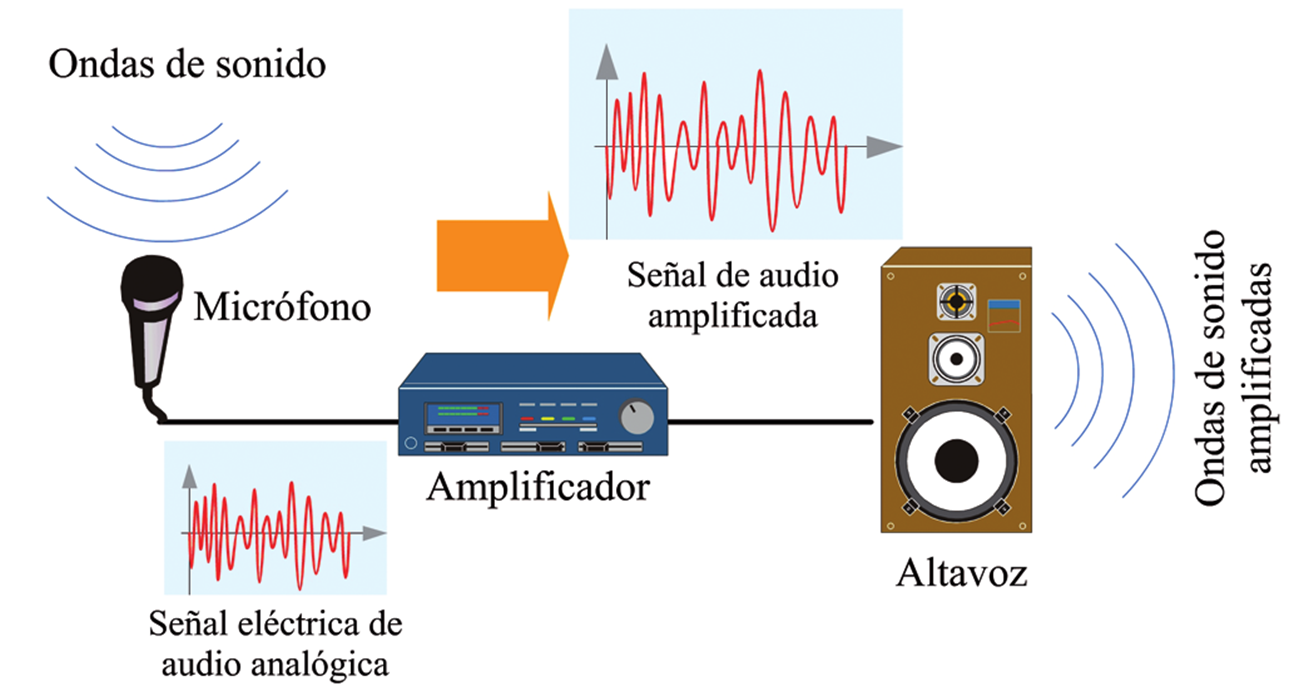
\includegraphics[width=0.82\textwidth]{image01.png}\\[8pt]
    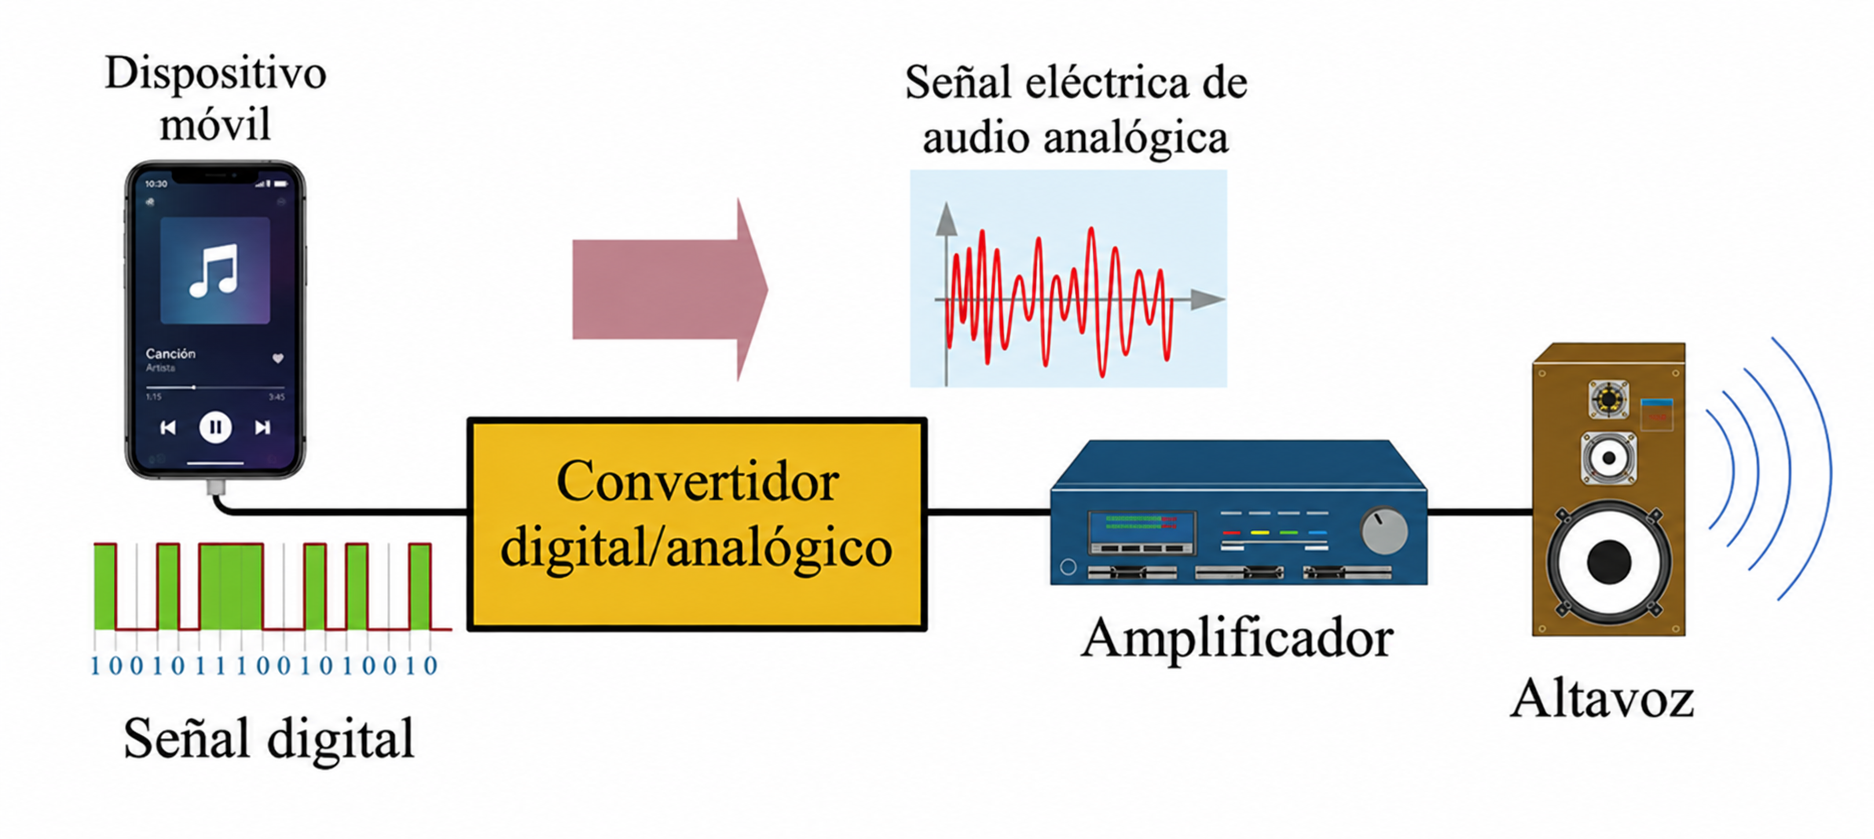
\includegraphics[width=0.82\textwidth]{image02.png}
    \caption{Sistema de audio con procesamiento analógico y digital.}
    \label{fig:audio}
\end{figure}

\subsection{Corriente eléctrica}

El movimiento de electrones que se establece en un conductor se llama corriente $i(t)$. La
corriente puede ser corriente continua (CC --- DC) o corriente alterna (CA --- AC), como se
aprecia en la figura~\ref{fig:cacc}. La unidad de la corriente es el ampere (\unit{\ampere}).

\begin{figure}[H]
    \centering
    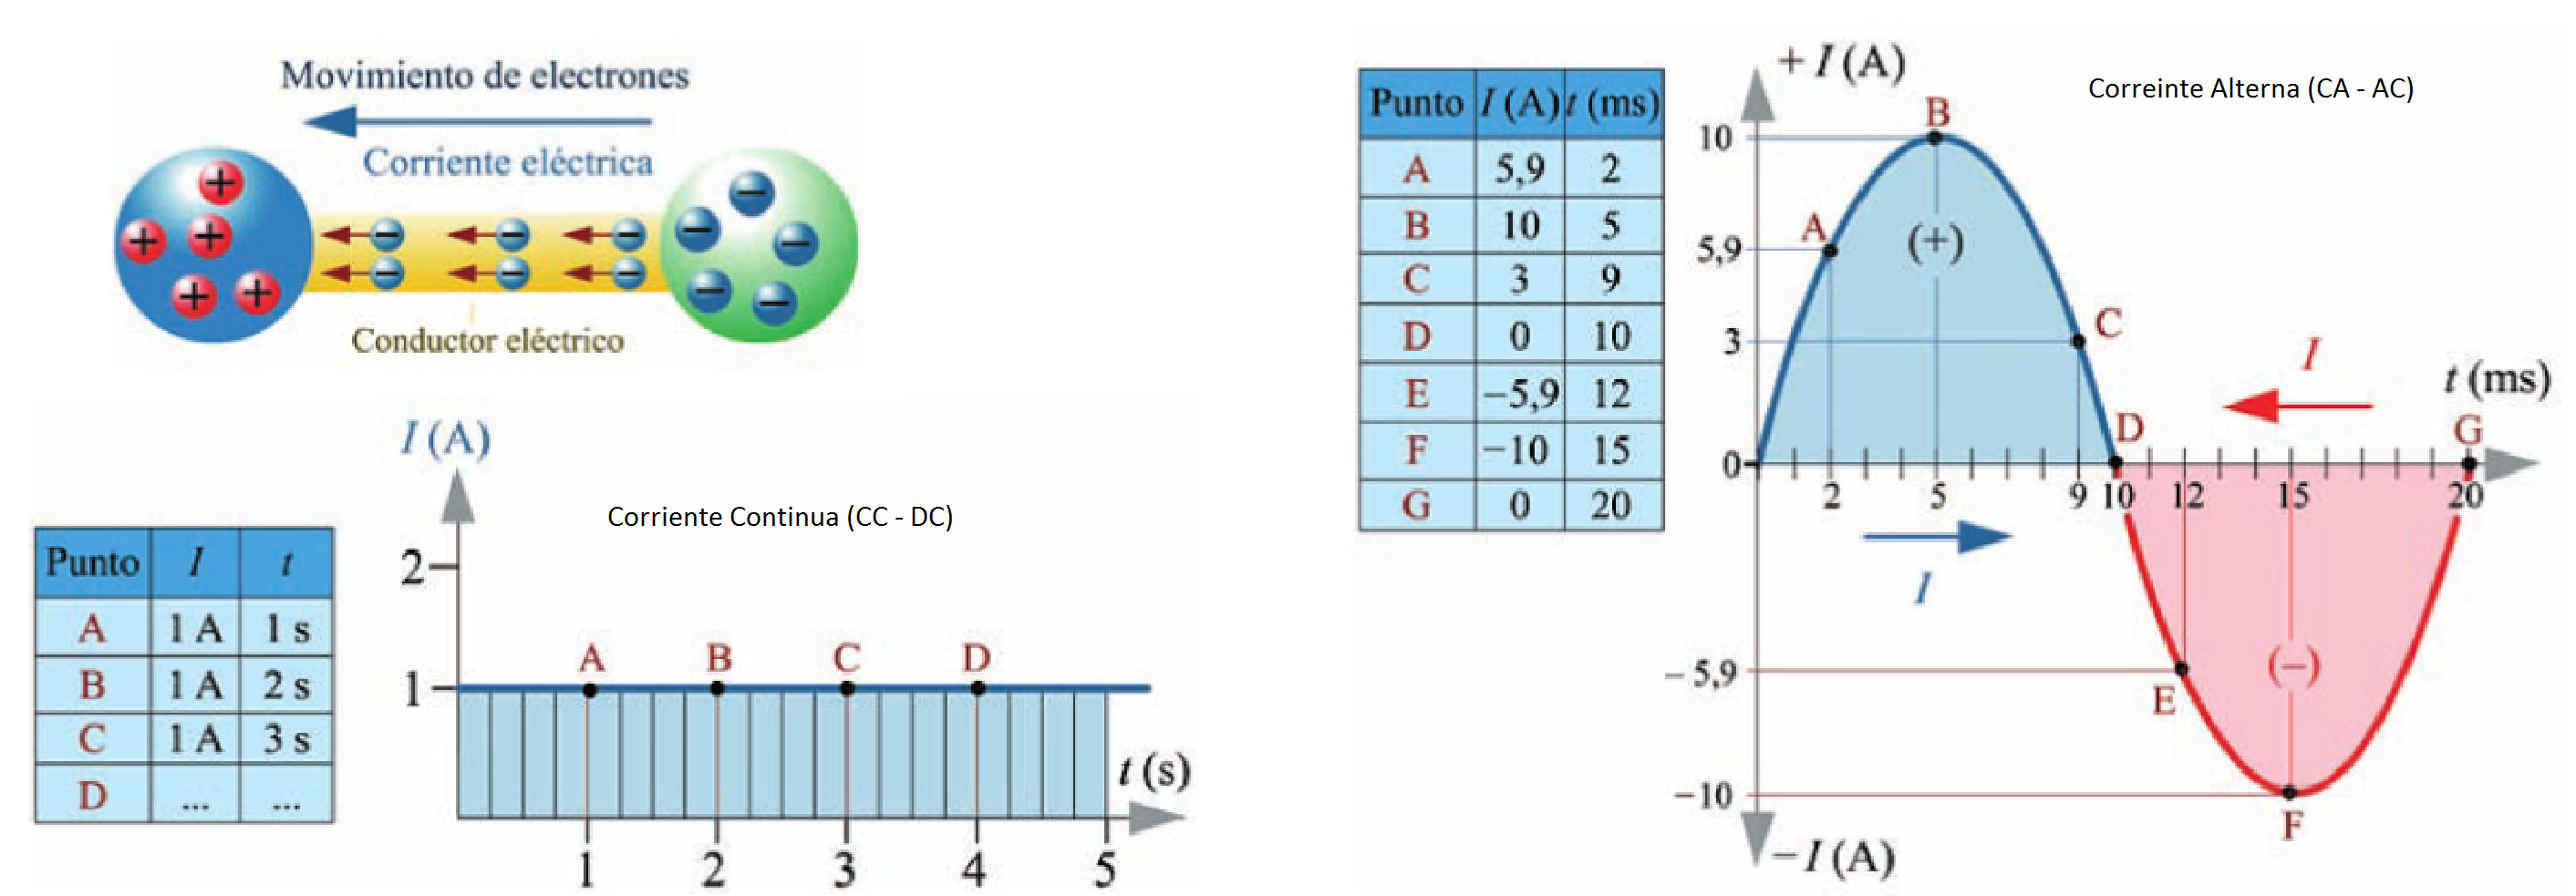
\includegraphics[width=0.92\textwidth]{image03.png}
    \caption{Corriente alterna \emph{vs.} corriente continua.}
    \label{fig:cacc}
\end{figure}

\begin{notatec}{notación y sentido de la corriente}
La corriente es el flujo de carga por unidad de tiempo:
\[
    i(t)=\frac{\mathrm{d}q}{\mathrm{d}t},
    \qquad
    \qty{1}{\ampere}=\qty{1}{\coulomb\per\second}.
\]
Se usa \textbf{minúscula} $i(t)$, $v(t)$ para valores \emph{instantáneos} (señales que varían en
el tiempo) y \textbf{mayúscula} $I$, $V$ para valores \emph{constantes} de continua. En todo este
curso se emplea el \emph{sentido convencional} de la corriente (del $+$ al $-$ por el circuito
externo), que es opuesto al movimiento real de los electrones.
\end{notatec}

\subsection{Tensión eléctrica y fuerza electromotriz}

Para generar una corriente es necesario que aparezca una fuerza capaz de mover los electrones
libres del circuito, que se denomina FEM (fuerza electromotriz --- fuente), ver
figura~\ref{fig:fuente}. Esta genera una tensión eléctrica o diferencia de potencial (también
denominada voltaje $V$), que es una magnitud física que cuantifica la diferencia de potencial
eléctrico entre dos puntos. Su unidad de medida es el voltio (\unit{\volt}).

\begin{figure}[H]
    \centering
    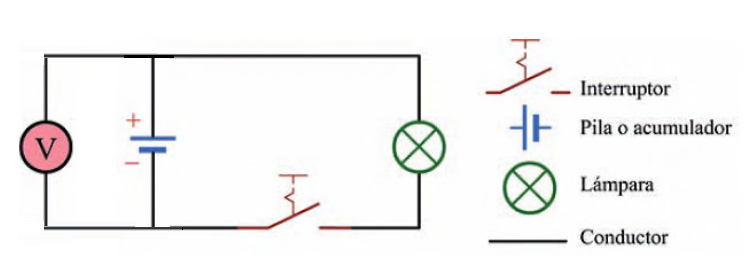
\includegraphics[width=0.55\textwidth]{image04.png}
    \caption{Fuente de tensión (voltaje) en un circuito eléctrico.}
    \label{fig:fuente}
\end{figure}

Un circuito eléctrico está compuesto por conductores y aislantes; los conductores permiten el
paso de corriente con facilidad, mientras que los aislantes bloquean el paso de la corriente.
En la figura~\ref{fig:cable} podemos observar la constitución de los cables eléctricos que
utilizaremos en la práctica, el cual está formado por un cable metálico de cobre (conductor) y un
recubrimiento de plástico (aislante), que evita que la corriente fugue a otro lugar no deseado.

\begin{figure}[H]
    \centering
    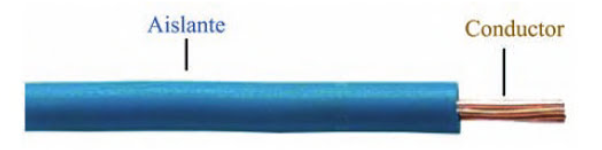
\includegraphics[width=0.55\textwidth]{image05.png}
    \caption{Partes de un cable eléctrico.}
    \label{fig:cable}
\end{figure}

\subsection{Resistencia eléctrica y ley de Ohm}

La resistencia eléctrica es una medida de la cantidad de oposición que ofrecen los cuerpos al
paso de la corriente. Su unidad de medida es el ohm y está representada por la letra griega
omega $\Omega$; los esquemáticos y modelos de las resistencias se pueden ver en la
figura~\ref{fig:resist}.

\begin{figure}[H]
    \centering
    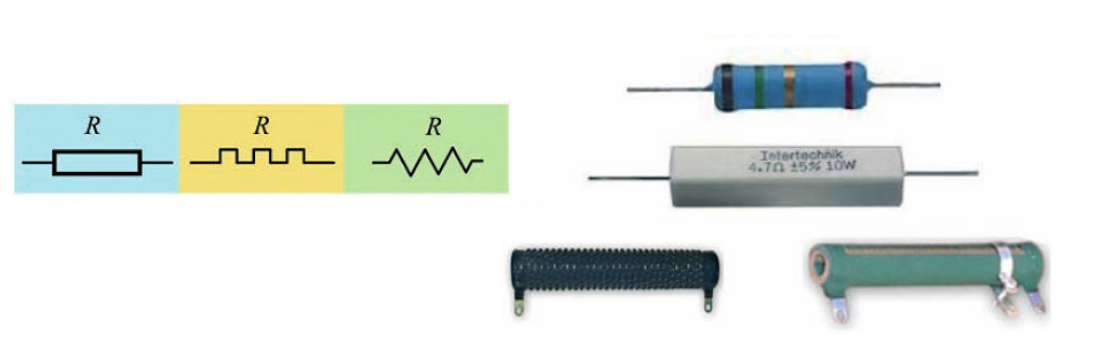
\includegraphics[width=0.82\textwidth]{image06.png}
    \caption{Símbolos y modelos de resistencias eléctricas.}
    \label{fig:resist}
\end{figure}

El físico alemán Ohm, mediante un experimento, descubrió que la intensidad de corriente que
recorre un circuito eléctrico es directamente proporcional a la tensión aplicada e inversamente
proporcional a la resistencia eléctrica, como se puede ver en la figura~\ref{fig:ohm}:

\begin{equation}
    I=\frac{V}{R}
    \qquad\Longleftrightarrow\qquad
    V=I\,R
    \qquad\Longleftrightarrow\qquad
    R=\frac{V}{I}
    \label{eq:ohm}
\end{equation}

\begin{figure}[H]
    \centering
    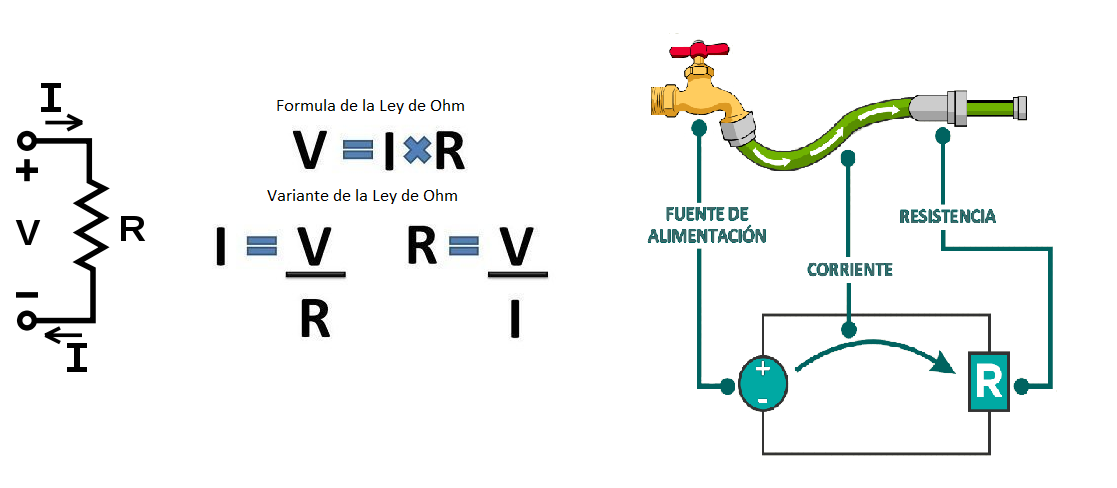
\includegraphics[width=0.78\textwidth]{image07.png}
    \caption{La ley de Ohm y su interpretación.}
    \label{fig:ohm}
\end{figure}

\begin{notatec}{la resistencia también disipa potencia}
Toda resistencia recorrida por una corriente convierte energía eléctrica en calor. La potencia
disipada es
\begin{equation}
    P = V\,I = I^{2}R = \frac{V^{2}}{R},
    \label{eq:potencia}
\end{equation}
y se mide en watts (\unit{\watt}). Elegir el valor óhmico \emph{no} es suficiente: también hay
que elegir la \textbf{potencia nominal} del componente. Las resistencias de película de carbón
del laboratorio son típicamente de \qty{0.25}{\watt}; si el cálculo con
la ecuación~\eqref{eq:potencia} da un valor mayor, la resistencia se quemará.
\end{notatec}

\subsection{Tolerancia y código de colores}

Las resistencias se fabrican con diferentes valores óhmicos, pero es muy difícil fabricar una
resistencia con un valor exacto; mientras más exacta sea la resistencia más se encarece el precio
del producto. De aquí nace el concepto de \textbf{tolerancia}, que indica los valores máximo y
mínimo de la resistencia:

\begin{equation}
    R_{\max}=R_{\text{nom}}\,(1+t),
    \qquad
    R_{\min}=R_{\text{nom}}\,(1-t).
    \label{eq:tol}
\end{equation}

Para entender mejor la exactitud de la resistencia, en la figura~\ref{fig:carbon} se aprecia el
modelo de resistencia de carbón, que es la más usada para pequeñas potencias. La resistencia
consiste en un cilindro aislado en el que se deposita una película delgada de carbón entre 2
conductores metálicos en los extremos; para obtener una resistencia determinada se realiza una
excavación helicoidal a lo largo de la película de carbón.

\begin{figure}[H]
    \centering
    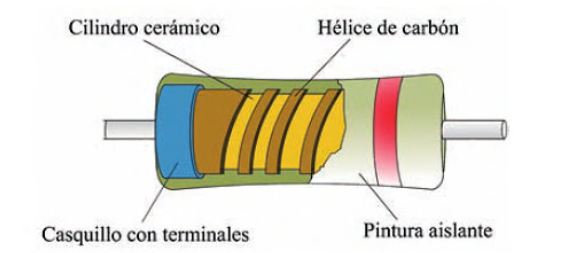
\includegraphics[width=0.5\textwidth]{image08.png}
    \caption{Resistencia de película de carbón.}
    \label{fig:carbon}
\end{figure}

Los valores comerciales de las resistencias se representan a través de una serie de anillos de
colores pintados sobre la superficie esmaltada de la resistencia, que se leen de acuerdo a la
figura~\ref{fig:colores}.

\begin{figure}[H]
    \centering
    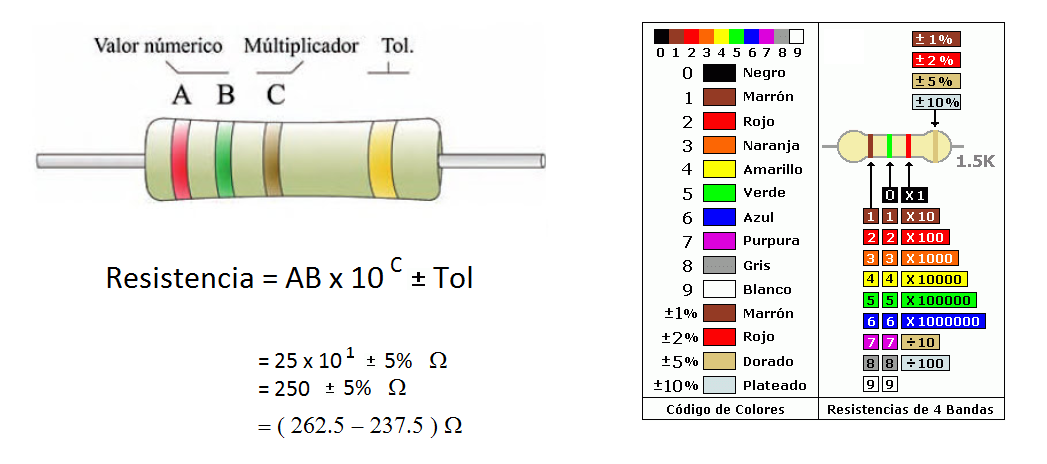
\includegraphics[width=0.82\textwidth]{image09.png}
    \caption{Ejemplo de lectura de resistencia.}
    \label{fig:colores}
\end{figure}

\begin{table}[H]
    \centering
    \caption{Código de colores de 4 bandas (referencia para el cuestionario previo).}
    \label{tab:colores}
    \small
    \begin{tabular}{lccc}
    \toprule
    \textbf{Color} & \textbf{Bandas 1 y 2 (dígito)} & \textbf{Banda 3 (multiplicador)} &
    \textbf{Banda 4 (tolerancia)}\\
    \midrule
    Negro     & 0 & $\times 10^{0}$  & ---\\
    Marrón    & 1 & $\times 10^{1}$  & $\pm\qty{1}{\percent}$\\
    Rojo      & 2 & $\times 10^{2}$  & $\pm\qty{2}{\percent}$\\
    Naranja   & 3 & $\times 10^{3}$  & ---\\
    Amarillo  & 4 & $\times 10^{4}$  & ---\\
    Verde     & 5 & $\times 10^{5}$  & $\pm\qty{0.5}{\percent}$\\
    Azul      & 6 & $\times 10^{6}$  & $\pm\qty{0.25}{\percent}$\\
    Violeta   & 7 & $\times 10^{7}$  & $\pm\qty{0.1}{\percent}$\\
    Gris      & 8 & $\times 10^{8}$  & $\pm\qty{0.05}{\percent}$\\
    Blanco    & 9 & $\times 10^{9}$  & ---\\
    Dorado    & --- & $\times 10^{-1}$ & $\pm\qty{5}{\percent}$\\
    Plateado  & --- & $\times 10^{-2}$ & $\pm\qty{10}{\percent}$\\
    Sin banda & --- & ---              & $\pm\qty{20}{\percent}$\\
    \bottomrule
    \end{tabular}
\end{table}

\begin{ejemplo}{lectura de una resistencia de \qty{330}{\ohm}}
Bandas: \textbf{naranja--naranja--marrón--dorado}.
\[
    R_{\text{nom}} = 33 \times 10^{1}\,\unit{\ohm} = \qty{330}{\ohm},
    \qquad t = \qty{5}{\percent}.
\]
Aplicando la ecuación~\eqref{eq:tol}:
\[
    R_{\max}=\qty{330}{\ohm}\times 1{,}05=\qty{346.5}{\ohm},
    \qquad
    R_{\min}=\qty{330}{\ohm}\times 0{,}95=\qty{313.5}{\ohm}.
\]
Es decir, el fabricante garantiza únicamente que el valor real está en el intervalo
\qtyrange{313.5}{346.5}{\ohm}.
\end{ejemplo}

\FloatBarrier
\subsection{El diodo LED}

Otro componente que utilizaremos en la práctica será el diodo luminiscente LED, utilizado en gran
medida como señalizador de encendido en equipos electrónicos. El diodo presenta 2 terminales, el
ánodo y el cátodo: el ánodo físicamente presenta una patilla más larga y en su símbolo la patilla
se conecta a la base de un triángulo; en el terminal del cátodo se ha diseñado el LED con un
pequeño aplanamiento y el símbolo de la patilla presenta una raya. Esto se puede apreciar en la
figura~\ref{fig:led}. Para que funcione un LED se debe aplicar por lo menos entre
\qtyrange{1.5}{2.2}{\volt} y una corriente comprendida entre \qtyrange{10}{50}{\milli\ampere}.

\begin{figure}[H]
    \centering
    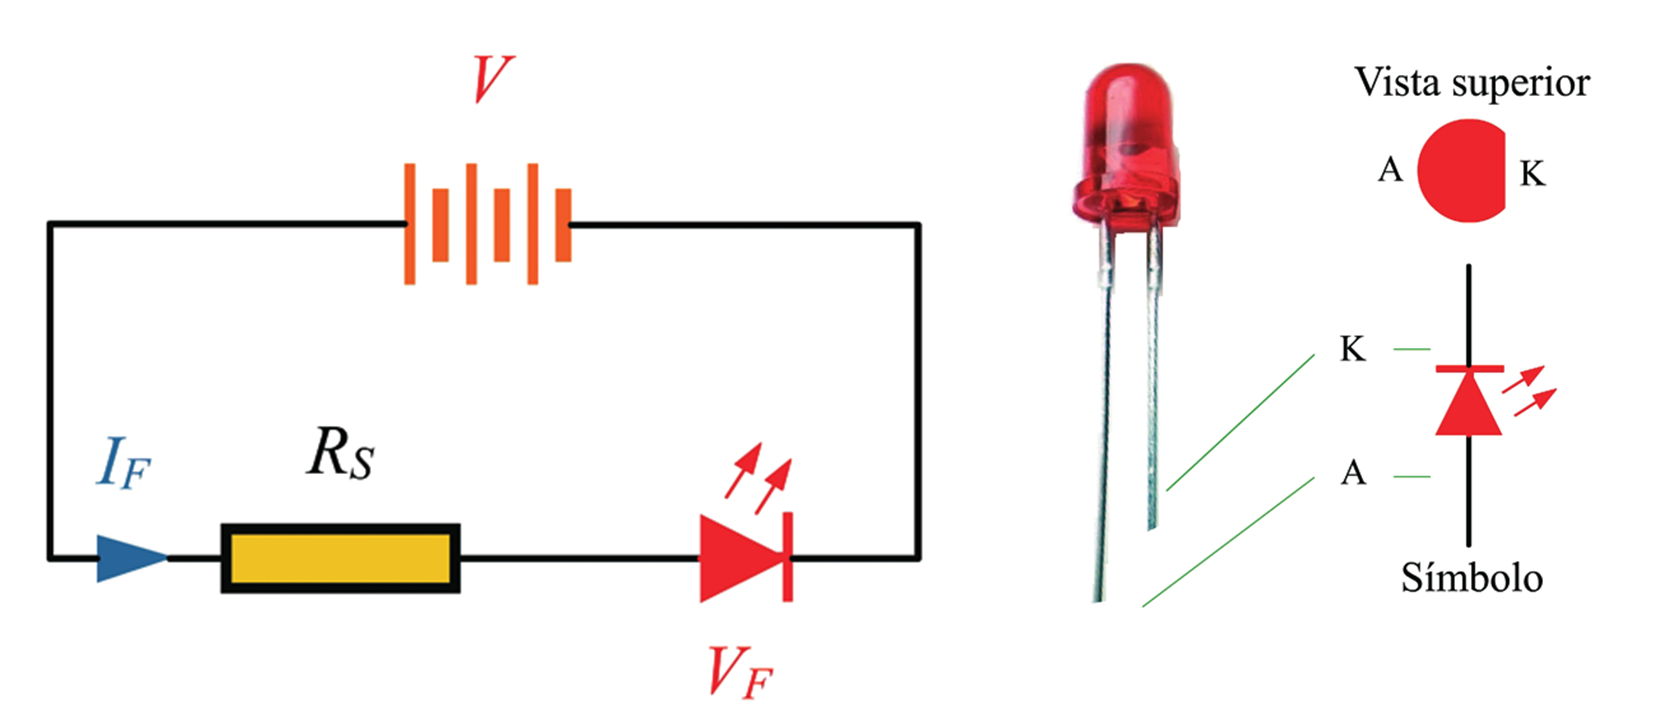
\includegraphics[width=0.85\textwidth]{image10.png}
    \caption{Símbolo y conexionado de un diodo LED.}
    \label{fig:led}
\end{figure}

\begin{notatec}{el LED nunca se conecta directamente a la fuente}
El LED es un dispositivo \textbf{no lineal}: por encima de su tensión umbral $V_F$ la corriente
crece de forma exponencial con la tensión, por lo que \emph{no} obedece la ley de Ohm y una
pequeña variación de tensión lo destruye. Por eso siempre se coloca una \textbf{resistencia
limitadora} $R_S$ en serie, cuyo valor se obtiene aplicando la ley de Ohm a la caída restante:
\begin{equation}
    R_S=\frac{V_{CC}-V_F}{I_F}.
    \label{eq:rled}
\end{equation}
Valores típicos: $V_F \approx$~\qtyrange{1.8}{2.2}{\volt} (rojo),
$V_F \approx$~\qtyrange{3.0}{3.4}{\volt} (azul, verde, blanco). En cuanto a la corriente, el
rango de \qtyrange{10}{50}{\milli\ampere} citado arriba corresponde a LED de potencia: un LED
indicador estándar de \qty{5}{\milli\meter} admite como \textbf{máximo continuo}
\qty{20}{\milli\ampere}, y trabaja perfectamente con \qtyrange{5}{15}{\milli\ampere}. Diseñe
siempre en ese rango salvo que la hoja de datos del componente indique otra cosa.
\end{notatec}

\begin{ejemplo}{resistencia limitadora del circuito de la práctica}
Se desea encender un LED rojo ($V_F \approx \qty{2}{\volt}$) desde la fuente fija de la EEB
($V_{CC}=\qty{5}{\volt}$) con la resistencia de \qty{330}{\ohm} de la actividad~2. Usando la
ecuación~\eqref{eq:rled} en sentido inverso:
\[
    I_F=\frac{V_{CC}-V_F}{R_S}=\frac{\qty{5}{\volt}-\qty{2}{\volt}}{\qty{330}{\ohm}}
       =\qty{9.1}{\milli\ampere}.
\]
Potencia disipada en la resistencia, según la ecuación~\eqref{eq:potencia}:
\[
    P_R=I_F^{2}R_S=(\qty{9.1}{\milli\ampere})^{2}\times\qty{330}{\ohm}
       =\qty{27.3}{\milli\watt}\ll\qty{0.25}{\watt}.
\]
La corriente está dentro del rango seguro y la resistencia de \qty{0.25}{\watt} trabaja muy
holgada: el diseño es correcto.
\end{ejemplo}

\FloatBarrier
\subsection{La placa protoboard}

Finalmente tocaremos el tema del \emph{protoboard} o placa de montaje rápido. Estas placas poseen
una serie de orificios interconectados entre sí, como se muestra en la figura~\ref{fig:proto}, en
donde se pueden conectar los dispositivos electrónicos y se pueden realizar todo tipo de
circuitos; las filas superiores e inferiores se suelen utilizar para conectar la tensión de
alimentación del circuito.

\begin{figure}[H]
    \centering
    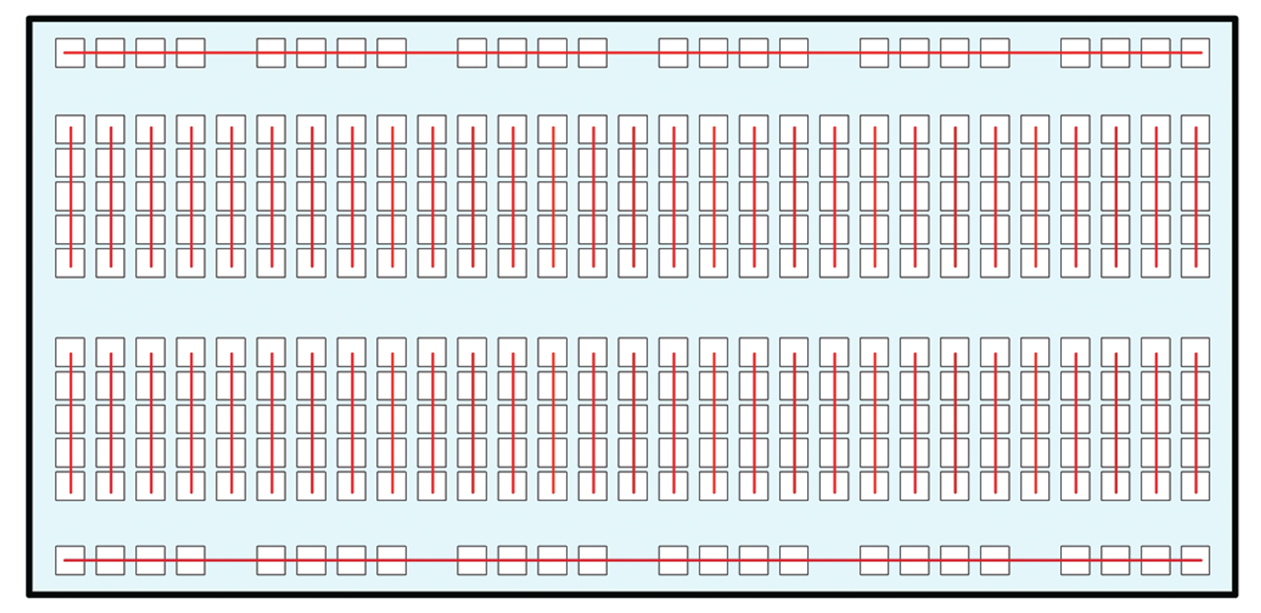
\includegraphics[width=0.8\textwidth]{image11.png}
    \caption{Esquema de conexionado de una placa protoboard.}
    \label{fig:proto}
\end{figure}

\begin{notatec}{cómo está conectada internamente}
Las dos filas horizontales del borde son los \textbf{buses de alimentación} y están unidas a lo
largo de toda la placa. En la zona central, cada columna de cinco orificios está unida
verticalmente, y el \textbf{canal central} separa eléctricamente las dos mitades: ese canal
existe para que un circuito integrado DIP quede montado a caballo sin cortocircuitar sus patillas
opuestas. Dos componentes conectados en la misma columna quedan en el \emph{mismo nodo}
eléctrico; para conectarlos en serie deben ocupar columnas distintas.
\end{notatec}

\FloatBarrier
%=======================================================================
\section{Cuestionario previo}
%=======================================================================
\begin{enumerate}
\item Complete la siguiente tabla usando la ley de Ohm, ecuación~\eqref{eq:ohm}.

\begin{table}[H]
    \centering
    \renewcommand{\arraystretch}{1.45}
    \begin{tabular}{|>{\centering\arraybackslash}m{2cm}|>{\centering\arraybackslash}m{2.6cm}
                    |>{\centering\arraybackslash}m{2.6cm}|>{\centering\arraybackslash}m{2.6cm}|}
    \hline
    \textbf{Ejercicio} & \textbf{I} & \textbf{V} & \textbf{R}\\
    \hline
    1 & \qty{1}{\ampere}        & \qty{5}{\volt}         & \\
    \hline
    2 & \qty{2}{\ampere}        &                        & \qty{5}{\kilo\ohm}\\
    \hline
    3 & \qty{300}{\milli\ampere}& \qty{20}{\milli\volt}  & \\
    \hline
    4 &                         & \qty{1}{\kilo\volt}    & \qty{10}{\kilo\ohm}\\
    \hline
    5 &                         & \qty{5}{\volt}         & \qty{330}{\ohm}\\
    \hline
    \end{tabular}
\end{table}

\item Escoja 4 resistencias diferentes y complete la siguiente tabla. Use el código de colores de
la tabla~\ref{tab:colores} y la ecuación~\eqref{eq:tol}.

\begin{table}[H]
    \centering
    \footnotesize
    \renewcommand{\arraystretch}{1.7}
    \begin{tabular}{|>{\centering\arraybackslash}m{1.35cm}|>{\centering\arraybackslash}m{1.35cm}
                    |>{\centering\arraybackslash}m{1.35cm}|>{\centering\arraybackslash}m{1.35cm}
                    |>{\centering\arraybackslash}m{1.35cm}|>{\centering\arraybackslash}m{1.8cm}
                    |>{\centering\arraybackslash}m{1.6cm}|>{\centering\arraybackslash}m{2.4cm}|}
    \hline
    \textbf{Ejer\-cicio} & \textbf{Color 1} & \textbf{Color 2} & \textbf{Color 3} &
    \textbf{Color 4} & \textbf{Valor de resistencia} & \textbf{Tole\-rancia} &
    \textbf{Resistencia (máx.\ --- mín.)}\\
    \hline
    1 & & & & & & & \\
    \hline
    2 & & & & & & & \\
    \hline
    3 & & & & & & & \\
    \hline
    4 & & & & & & & \\
    \hline
    \end{tabular}
\end{table}

\item Describa con sus propias palabras qué es una bocina y cómo funciona.

\lineasresp{4}
\end{enumerate}

\FloatBarrier
%=======================================================================
\section{Equipos y materiales}
%=======================================================================
\noindent\textbf{Laboratorio:} Electrónica y Comunicaciones.

\vspace{0.25cm}
\noindent\textbf{Equipos y dispositivos:}
\begin{itemize}
    \item 1 computador personal.
    \item 1 Electronics Explorer Board (EEB).
    \item 1 diodo LED.
    \item 2 resistencias (una de \qty{330}{\ohm} para la actividad~2).
    \item 1 potenciómetro.
\end{itemize}

\noindent\textbf{Software:}
\begin{itemize}
    \item WaveForms.
\end{itemize}

\FloatBarrier
%=======================================================================
\section{Actividades}
%=======================================================================
\subsection{Actividad: conectando la Electronics Explorer Board}

\begin{enumerate}[label=\textbf{\Alph*.}, leftmargin=*, labelsep=0.6em, series=acteeb]
\item La \emph{Electronics Explorer Board} es un sistema de medición todo en uno, que sirve para
diseñar y probar circuitos analógicos y digitales. Está construida en base a 2 placas protoboard
y permite el prototipado rápido y simple de circuitos. La operación de la EE Board es fácil de
manejar a través del software WaveForms de Digilent; los componentes de la tarjeta se pueden
observar en la figura~\ref{fig:eeb}.
\end{enumerate}

\begin{figure}[H]
    \centering
    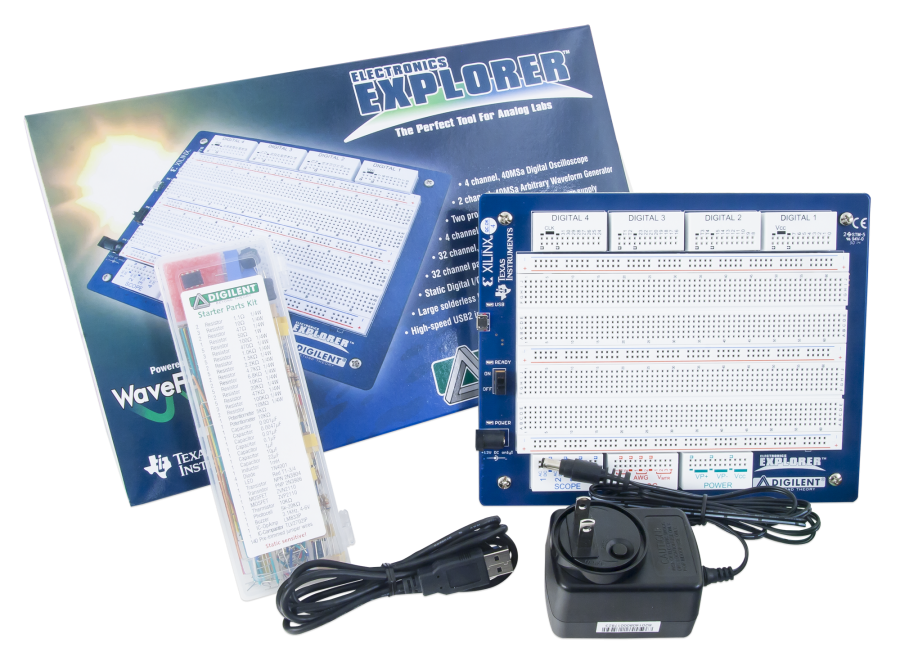
\includegraphics[width=0.72\textwidth]{image12.png}
    \caption{Componentes de la tarjeta EE Board.}
    \label{fig:eeb}
\end{figure}

\begin{enumerate}[resume*=acteeb]
\item La comunicación con la EE Board se realiza a través de una conexión USB y la interconexión
es bastante simple. Se utiliza un cable micro-USB para conectar la tarjeta a un ordenador. La EE
Board también tiene un adaptador de \emph{jack} de alimentación de \qty{12}{\volt} de energía
externa. Con el cable USB y la fuente de alimentación externa conectada, girar el interruptor de
la tarjeta a \textbf{ON}, lo cual prepara a la EE Board para la comunicación con el software
WaveForms. Esta conexión se puede apreciar en la figura~\ref{fig:conex}.
\end{enumerate}

\begin{figure}[H]
    \centering
    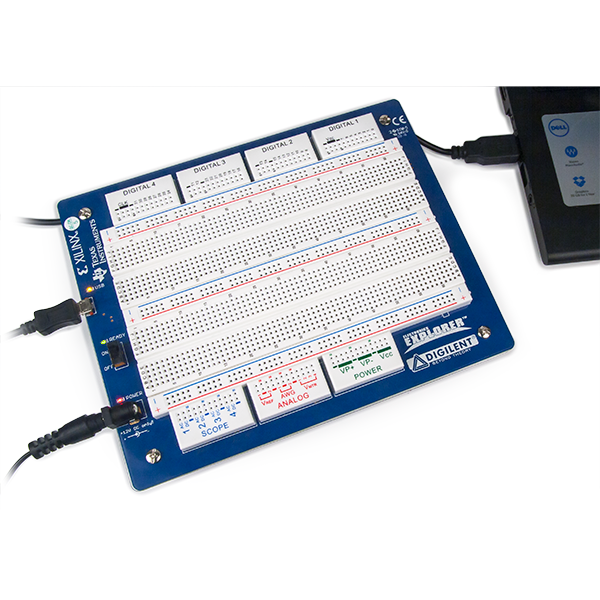
\includegraphics[width=0.52\textwidth]{image13.png}
    \caption{Conexionado de la tarjeta EE Board.}
    \label{fig:conex}
\end{figure}

\begin{enumerate}[resume*=acteeb]
\item Las partes que conforman la tarjeta se pueden separar en 3 grupos, que son: la zona de
instrumentos, la tarjeta protoboard o \emph{breadboard} y la zona de conexiones digitales. Esto
se aprecia en la figura~\ref{fig:grupos}.
\end{enumerate}

\begin{figure}[H]
    \centering
    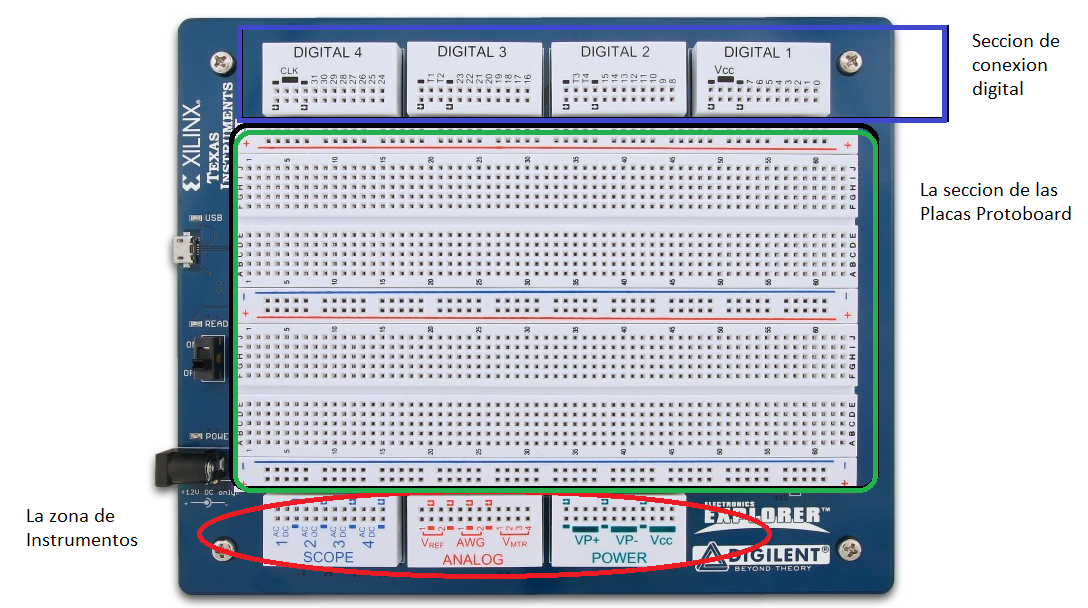
\includegraphics[width=0.78\textwidth]{image14.png}
    \caption{Grupos de partes que conforman la tarjeta EE Board.}
    \label{fig:grupos}
\end{figure}

% Caracteristicas de la EE Board, agrupadas en TRES bloques, uno por panel
% fisico de la tarjeta:
%
%   SCOPE   -> osciloscopio
%   ANALOG  -> AWG, voltimetro (VMTR) y voltajes de referencia (VREF)
%   POWER   -> fuente variable (VP+/VP-) y fuente fija (Vcc)
%
% Cada bloque es UNA fila: la imagen de la derecha ilustra todo lo que hay a su
% izquierda. Por eso VMTR y VREF van con el AWG, y la fuente fija con la
% variable: aparecen juntos en el mismo panel de la placa.
%
% Las siete caracteristicas llevan el marcador de primer nivel (\labelitemi, el
% cuadradito) forzado con la opcion label: como el bloque vive dentro de una
% enumerate, LaTeX les habria puesto por defecto el marcador de segundo nivel.
% Las sublistas "Donde:" si usan el de segundo nivel, para que se distingan.
%
% La tabla va DENTRO del \item para heredar la sangria y quedar alineada con el
% resto del contenido; de ahi que se dimensione con \linewidth y no \textwidth.
% Es una tabularx SIN filetes, cabecera ni \caption: solo alinea las columnas,
% y no se envuelve en un entorno table para que no reciba numeracion de cuadro.
\begin{enumerate}[resume*=acteeb]
\item Específicamente, la EE Board cuenta con:

\begingroup
\setlength{\tabcolsep}{0pt}
\renewcommand{\arraystretch}{1.2}
\setlist[itemize]{itemsep=2pt,topsep=4pt,parsep=0pt}
% marcador de cuadradito, con sangria colgante
\newlist{carac}{itemize}{1}
\setlist[carac]{label=\labelitemi, leftmargin=1.5em, topsep=0pt, itemsep=0pt}
\newcommand{\dentroeeb}{0.32cm}

\vspace{0.4cm}
\noindent
\begin{tabularx}{\linewidth}{@{}>{\raggedright\arraybackslash}X@{\hspace{0.7cm}}>{\centering\arraybackslash}p{4.0cm}@{}}

%------------------------------------------------- bloque 1: SCOPE
\begin{carac}
\item \textbf{4 canales de osciloscopio a \qty{40}{\mega\sample\per\second},
      \qty{100}{\mega\hertz}.}

      Dónde:
      \begin{itemize}[leftmargin=1.4em]
          \item \textbf{AC}: canal sin \emph{offset} de voltaje.
          \item \textbf{DC}: canal con \emph{offset} de voltaje.
          \item \textbf{--}: es la tierra (referencia común).
      \end{itemize}
\end{carac}
&
\begin{minipage}[t]{\linewidth}\vspace{0pt}
    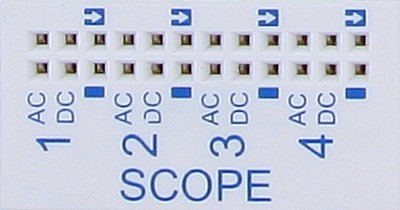
\includegraphics[width=\linewidth]{image15.png}
\end{minipage}
\\
\addlinespace[1.1cm]

%------------------------------------------------- bloque 2: ANALOG
\begin{carac}
\item \textbf{2 canales, \qty{40}{\mega\sample\per\second},
      \qty{20}{\mega\hertz}, generador de forma de onda arbitraria (AWG).}

      Dónde:
      \begin{itemize}[leftmargin=1.4em]
          \item \textbf{AWG 1}: primer canal.
          \item \textbf{AWG 2}: segundo canal.
          \item \textbf{--}: es la tierra.
      \end{itemize}

\vspace{\dentroeeb}
\item \textbf{4 canales de voltímetro (VMTR).}

\vspace{\dentroeeb}
\item \textbf{2 voltajes de referencia programables:} VREF~1 y VREF~2.
\end{carac}
&
\begin{minipage}[t]{\linewidth}\vspace{0pt}
    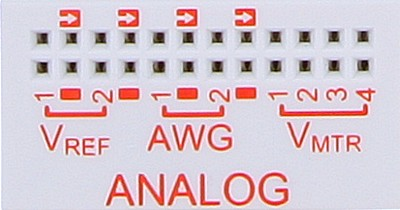
\includegraphics[width=\linewidth]{image16.png}
\end{minipage}
\\
\addlinespace[1.1cm]

%------------------------------------------------- bloque 3: POWER
\begin{carac}
\item \textbf{2 canales, \qty{\pm 9}{\volt}, \qty{1.5}{\ampere}, fuente de
      alimentación variable.}

      Dónde:
      \begin{itemize}[leftmargin=1.4em]
          \item \textbf{VP+}: es $+\qty{9}{\volt}$, \qty{1.5}{\ampere}.
          \item \textbf{VP--}: es $-\qty{9}{\volt}$, \qty{1.5}{\ampere}.
          \item \textbf{--}: es la tierra.
      \end{itemize}

\vspace{\dentroeeb}
\item \textbf{1 canal, \qty{3.3}{\volt}~/~\qty{5}{\volt}, \qty{2}{\ampere},
      fuente de alimentación fija ($V_{CC}$).}
\end{carac}
&
\begin{minipage}[t]{\linewidth}\vspace{0pt}
    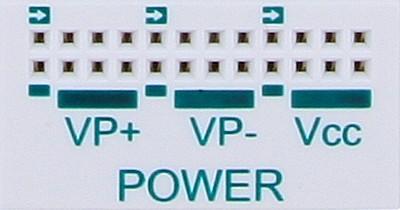
\includegraphics[width=\linewidth]{image17.png}
\end{minipage}
\\

\end{tabularx}

\vspace{0.45cm}

% Septima caracteristica: mismo marcador y misma jerarquia que las seis
% anteriores, aunque no lleve imagen que la acompane.
\begin{carac}
\item \textbf{Puede conectar 32 señales digitales,} que se pueden configurar
      como:
      \begin{itemize}[leftmargin=1.4em]
          \item Analizador lógico de 32 canales.
          \item Generador de patrones de 32 canales.
          \item E/S digitales discretas (botones, interruptores, LED, etc.).
      \end{itemize}
\end{carac}
\endgroup
\end{enumerate}

\begin{figure}[H]
    \centering
    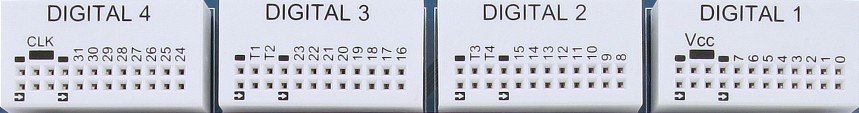
\includegraphics[width=0.9\textwidth]{image18.png}
    \caption{Zona de conexiones digitales de la EE Board.}
    \label{fig:digital}
\end{figure}





\begin{enumerate}[resume*=acteeb]
\item En cuanto al software WaveForms, antes de iniciarlo conecte la EE Board al ordenador,
conecte su transformador y encienda el \emph{switch} (ON); después ejecute el programa y le
aparecerá la imagen de la figura~\ref{fig:waveforms}. Acepte la configuración por defecto de la
EE Board.
\end{enumerate}

\begin{figure}[H]
    \centering
    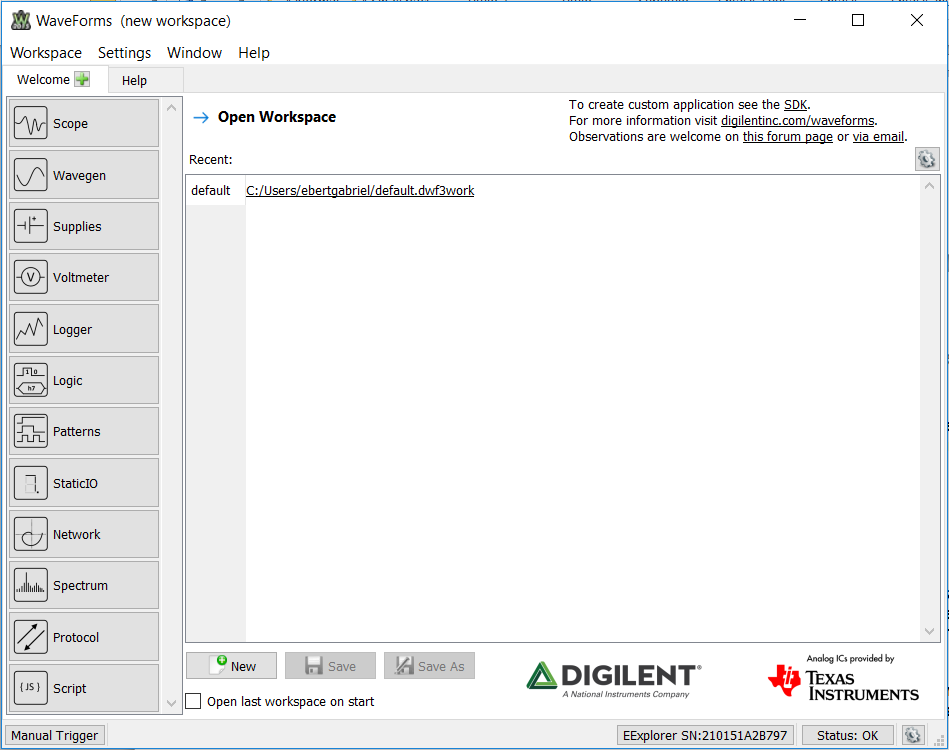
\includegraphics[width=0.68\textwidth]{image19.png}
    \caption{Pantalla de inicio del software WaveForms.}
    \label{fig:waveforms}
\end{figure}

\FloatBarrier
\subsection{Actividad: mi primer circuito}

\begin{enumerate}[label=\textbf{\Alph*.}, leftmargin=*, labelsep=0.6em, series=actcir]
\item En este primer circuito haremos simplemente un circuito serie que nos permitirá encender y
apagar un diodo LED. Para esto arme en la zona protoboard de la EE Board el circuito esquemático
mostrado en la figura~\ref{fig:esquema}; para tener una mejor perspectiva del circuito puede
revisar la figura~\ref{fig:implement}.
\end{enumerate}

\begin{figure}[H]
    \centering
    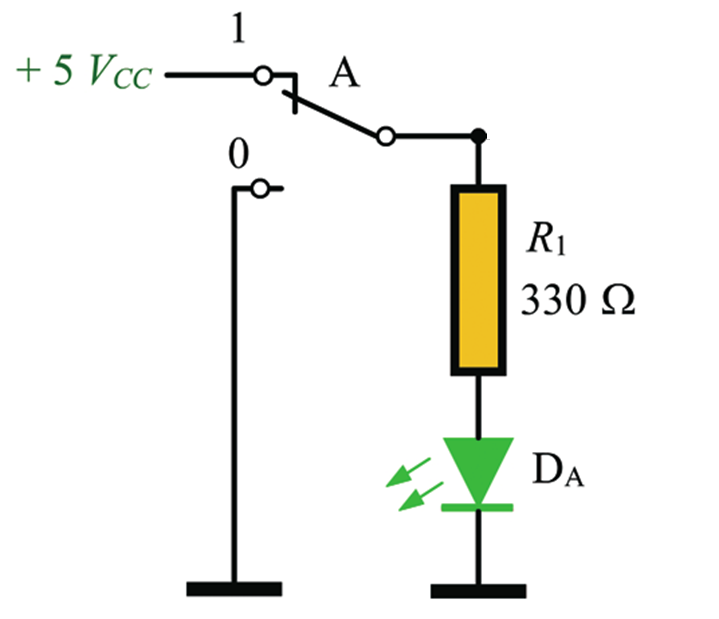
\includegraphics[width=0.45\textwidth]{image20.png}
    \caption{Esquemático del circuito a implementar.}
    \label{fig:esquema}
\end{figure}

\begin{enumerate}[resume*=actcir]
\item Configure el circuito de la figura~\ref{fig:implement} y tenga cuidado con las patillas de
conexión del LED; después configure el software: en la opción \emph{Static I/O} cambie el tipo de
\emph{switch} y pruebe que el LED enciende. Esto se puede apreciar en la
figura~\ref{fig:switch}.
\end{enumerate}

\begin{figure}[H]
    \centering
    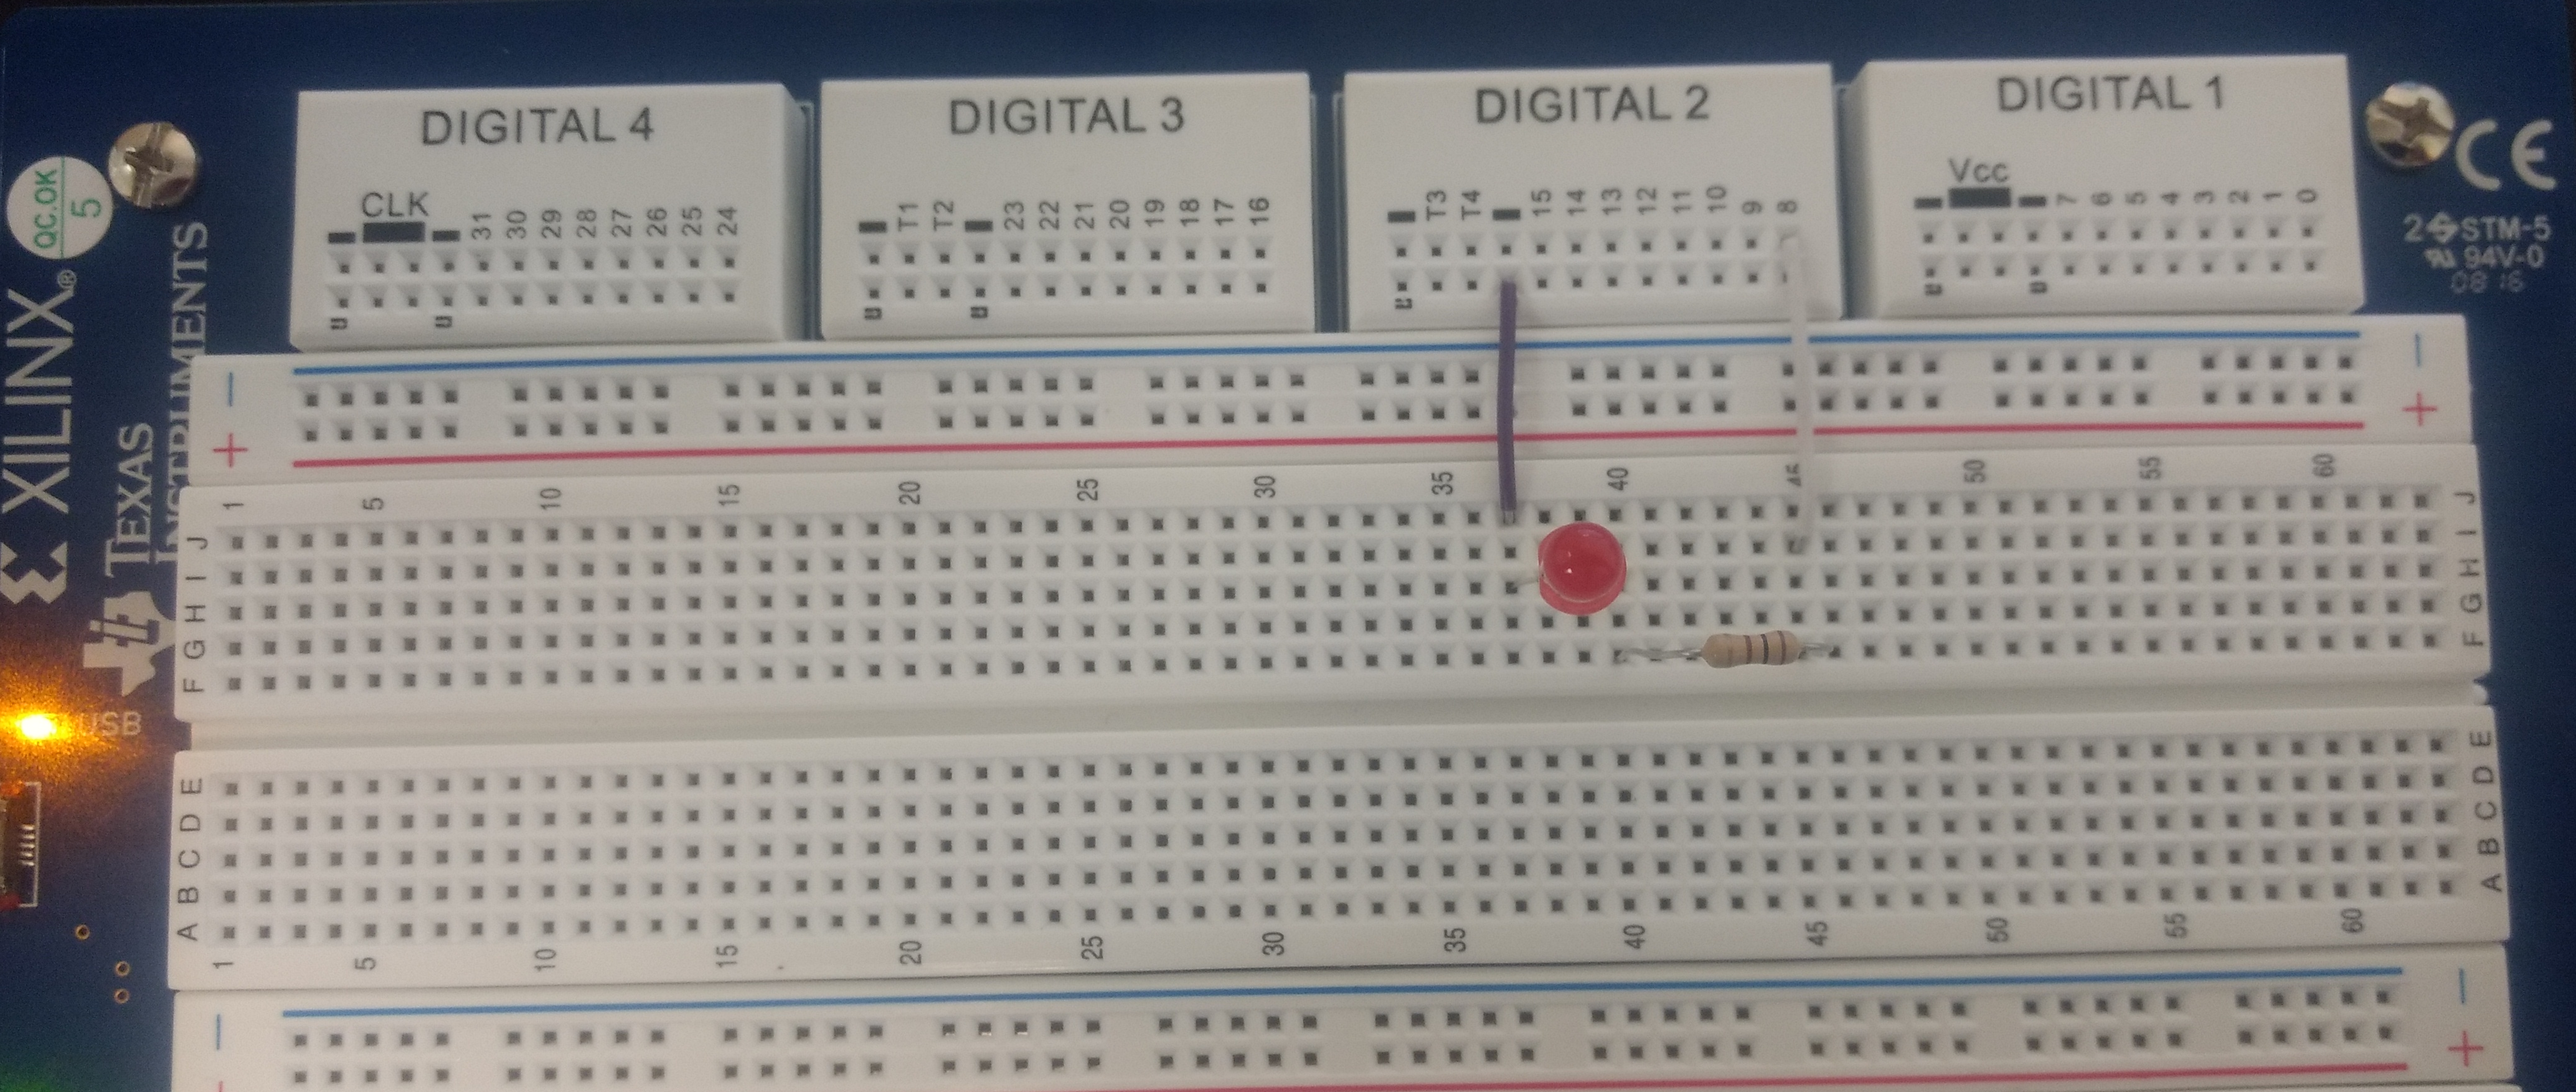
\includegraphics[width=\textwidth]{image21.png}
    \caption{Implementación del circuito en la EE Board.}
    \label{fig:implement}
\end{figure}

\begin{figure}[H]
    \centering
    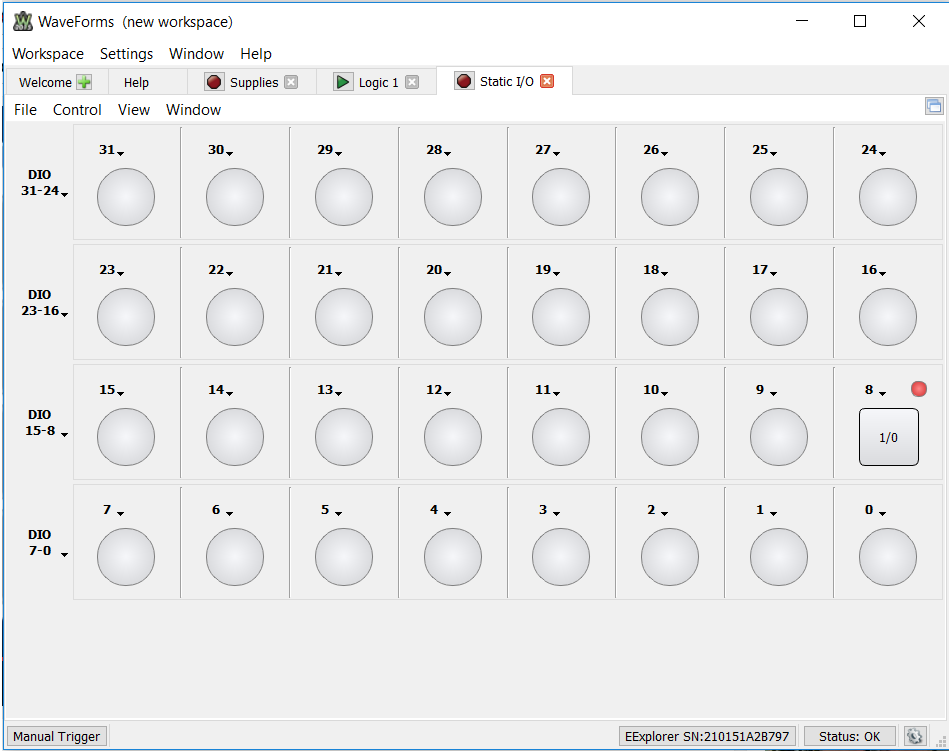
\includegraphics[width=0.68\textwidth]{image22.png}
    \caption{Configuración del \emph{switch} en el software WaveForms.}
    \label{fig:switch}
\end{figure}

\begin{notatec}{cómo funciona el interruptor de la figura~\ref{fig:esquema}}
El \emph{switch} no es un componente físico del protoboard: es una salida digital de la EE Board
gobernada desde la ventana \emph{Static I/O} de WaveForms. En la posición \textbf{1} la salida
entrega nivel alto ($\approx V_{CC}$) y circula corriente por $R_1$ y por el LED; en la posición
\textbf{0} entrega nivel bajo ($\approx \qty{0}{\volt}$) y el LED se apaga. Es el equivalente
digital de accionar un interruptor mecánico. Recuerde que una salida digital entrega una corriente
limitada (típicamente algunas decenas de \unit{\milli\ampere}), razón adicional para no bajar de
los \qty{330}{\ohm} de $R_1$.
\end{notatec}

\begin{ejemplo}{verificación experimental (recomendada)}
Con el circuito encendido, mida con el voltímetro (VMTR) de la EE Board y complete:

\vspace{4pt}
\centering
\renewcommand{\arraystretch}{1.5}
\begin{tabular}{|>{\centering\arraybackslash}m{4.6cm}|>{\centering\arraybackslash}m{2.6cm}
                |>{\centering\arraybackslash}m{2.6cm}|}
\hline
\textbf{Magnitud} & \textbf{Valor teórico} & \textbf{Valor medido}\\
\hline
$V_{CC}$ (fuente)                    & \qty{5}{\volt}          & \\
\hline
$V_{R_1}$ (sobre la resistencia)     & \qty{3}{\volt}          & \\
\hline
$V_F$ (sobre el LED)                 & $\approx\qty{2}{\volt}$ & \\
\hline
$I_F = V_{R_1}/R_1$                  & \qty{9.1}{\milli\ampere}& \\
\hline
\end{tabular}
\renewcommand{\arraystretch}{1}

\vspace{6pt}
\raggedright
Compruebe que se cumple la ley de tensiones de Kirchhoff: $V_{CC}=V_{R_1}+V_F$. Si la suma de
las tensiones medidas no coincide con la fuente, hay un contacto flojo en el protoboard.
\end{ejemplo}

\FloatBarrier
%=======================================================================
\section*{Referencias}
\addcontentsline{toc}{section}{Referencias}
%=======================================================================
\begin{enumerate}[label={[\arabic*]}]
    \item Digilent Inc., \emph{Electronics Explorer Board --- Reference Manual}.
          \url{https://digilent.com/reference/test-and-measurement/electronics-explorer/reference-manual}
    \item Digilent Inc., \emph{WaveForms --- Getting started with the Electronics Explorer Board}.
          \url{https://files.digilent.com/manuals/WaveForms/}
    \item IEC 60062, \emph{Marking codes for resistors and capacitors} (código de colores).
\end{enumerate}

\end{document}
